\documentclass[12pt]{report}

%%%%%%%%%%%%%%%%%%%%%%%%%%%%%%%%%%%%%%%%%%%%%%%%%%%%%%%%%%%%%%%%%%%%%%%%
\usepackage{pdfsync}        % allows clicking in PDF to take you back to the text

\usepackage{lmodern}        % use modern latin fonts
% \usepackage{palatino}        % use modern latin fonts
% \usepackage{times}        % use modern latin fonts
\usepackage[T1]{fontenc}    % use 8 bit output font encoding with more glyphs
\usepackage[utf8]{inputenc} % so you can type ă
% \usepackage{siunitx}        % automatically formats numbers with spaces and all that

\usepackage[dvipsnames]{xcolor}         % more color choices
\usepackage[english=british]{csquotes} % for correct use of `` '' ... TODO!!
\usepackage{url}            % typeset URL's sensibly
\usepackage[nottoc]{tocbibind} % include bibliography in ToC (third-rep.cls not working)
\usepackage{appendix} % customise the appearance of appendix via an 'appendix' environment

% \usepackage{tabu}
\usepackage{array}
\usepackage{colortbl}
\usepackage{colortbl}
\definecolor{LightGreen}{HTML}{9bffa0}

\usepackage{layouts} % allows you to print lengths

% set line space nicely (only for text, not captions etc)
\usepackage{setspace}
\onehalfspacing

\usepackage[a4paper,textwidth=159mm, hmargin ratio=1:1, vmargin ratio=1:1, verbose]{geometry}
\makeatletter
\AtEndPreamble{%
  \normalfont
  \ifcase \@ptsize
    \geometry{textheight=240mm}%
    \or
    \geometry{textheight=243mm}%
    \or
    \geometry{textheight=241mm}%
  \fi
}

\usepackage{enumitem} % configure labels of items in enumerations i.e. i), ii)
\setlist[description]{style=nextline,font=\normalfont\textbullet\space,labelindent=\parindent}


\usepackage{natbib}
\setcitestyle{authoryear,round}

% the starred \newcommand is more strick wrt the arguments it takes (cannot contain paragraph)
% so \newcommand* should be the default you use
\definecolor{ToDoColor}{rgb}{0.4,0.4,0.4}
\newcommand{\todo}[1]{\textcolor{ToDoColor}{ToDo: #1}}
\newcommand*{\startToDo}{\color{ToDoColor}ToDo: \\}
\newcommand*{\stopToDo}{\color{Black}}

%% =============================================================================
% Remove "Chapter x" line before a new chapter
% This should be in .cls file, ideally
\makeatletter
\renewcommand{\@makechapterhead}[1]{%
  % \vspace*{15 pt}% Space before the chapter name
  {\setlength{\parindent}{0pt} \raggedright \normalfont
    \bfseries\Huge
    #1% The chapter's name
    \par\nobreak\vspace{35 pt}}} % Space after chapter name
\makeatother
%% =============================================================================

\usepackage{amsmath, amssymb,mathtools,bm}
\usepackage{bbm}
\DeclareMathOperator*{\argmin}{argmin} % * means the argument in _{} is placed below rather than to the right
\DeclareMathOperator{\argmax}{argmax} % * means the argument in _{} is placed below rather than to the right
\DeclareMathOperator{\iou}{IoU}
\DeclareMathOperator{\AP}{\operatorname{AP}_{\iou > 0.5}}
\DeclareMathOperator{\cer}{CER}
\DeclareMathOperator{\wer}{WER}
\providecommand{\CER}[1]{\( \operatorname{CER} = #1\% \)}
\providecommand{\WER}[1]{\( \operatorname{WER} = #1\% \)}
\providecommand{\norm}[1]{\lVert#1\rVert} % unlike \newcommand, this does nothing if \norm already exists
\providecommand{\card}[1]{\left\vert#1\right\vert}
% \DeclarePairedDelimiter\norm{\lVert}{\rVert}
% \DeclarePairedDelimiter\card{\left\vert}{\right\vert}
\DeclarePairedDelimiter\ceil{\lceil}{\rceil}
\DeclarePairedDelimiter\floor{\lfloor}{\rfloor}

\newcommand*{\ve}[1]{\mathbf{#1}} % for displaying a vector
\newcommand*{\ma}[1]{\mathrm{#1}} % for displaying a matrix
\newcommand*{\cls}{\mathit{cls}} % for RPN loss
\newcommand*{\reg}{\mathit{reg}}
% this makes the symbol := look nicer
\mathchardef\ordinarycolon\mathcode`\:
\mathcode`\:=\string"8000
\begingroup \catcode`\:=\active
  \gdef:{\mathrel{\mathop\ordinarycolon}}
\endgroup


%----------------------------------------------------------------------------------------
\usepackage{graphicx}
  \graphicspath{{./images/}}
  \setkeys{Gin}{width=\linewidth} % set \includegraphics default width
  \makeatletter
    \let\ginnatwidth\Gin@nat@width
    \let\ginnatheight\Gin@nat@height
  \makeatother
  \usepackage[export]{adjustbox} % used to align some images with the text between them (valign=c)
%----------------------------------------------------------------------------------------

\usepackage[compatibility=false]{caption}
\usepackage{subcaption}
\usepackage{floatrow}       % automatically centers floats
  \newcommand{\rulesep}{\unskip\ \vrule\ } % allows to draw vertical line between figures

  % \subref -> '(a)' rather than just 'a'
  \captionsetup[subfigure]{subrefformat=simple,labelformat=simple}
  \renewcommand\thesubfigure{(\alph{subfigure})}
  \makeatletter
  \renewcommand\p@subfigure{\thefigure~}
  \makeatother

  % make the caption a bit shorter than the rest of the text, with bold font for label
  \captionsetup{margin=10pt,labelfont=bf,indention=.5cm}

  % include the short description into the long one
  \makeatletter
  \let\x@caption\caption % original \caption
  \def\x@@caption[#1]#2{\x@caption[{#1}]{#1 --- #2}} % with optional arg
  \def\x@@@caption#1{\x@caption[{#1}]{#1}} % without optional arg
  \AtBeginDocument{%
      \def\caption{\@ifnextchar[\x@@caption\x@@@caption} % new \caption
  }
  \makeatother


%----------------------------------------------------------------------------------------


\usepackage[backref]{hyperref}
\hypersetup{
  pdftitle      = {TODO},
  pdfauthor     = {Ciprian Tomoiaga},
  pdfsubject    = {TODO},
  pdfkeywords   = {TODO},
  pdfpagemode   = UseOutlines,
  pdfstartview  = Fit,
  pdfpagelayout = OneColumn,       % document in 1 column continuous scrolling
  unicode=true,                    % use Unicode in bookmarks
  bookmarksnumbered  = true,       % shows numbers in bookmarks like ToC
  bookmarksopen      = true,
  bookmarksopenlevel = 1,
  colorlinks   = true,             % Colours links instead of ugly boxes
  urlcolor     = {blue!80!black},  % Colour for external hyperlinks
  linkcolor    = {red!50!black},   % Colour of internal links
  citecolor    = {blue!50!black},  % Colour of citations
  breaklinks   = true,             % Break long links into lines
  linktocpage  = false             % ToC, LoF, LoT place hyperlink on page number, rather than entry text
}

%% ----------------------------------------------------------------------------
\newcommand*{\nolink}[1]{%
  \begin{NoHyper}#1\end{NoHyper}%
}

%% ----------------------------------------------------------------------------
\newcommand{\algorithmautorefname}{algorithm}
% TODO: workaround incompatibility hyperref + appendix package
% \newcommand{\appref}[1]{\hyperref[#1]{Appendix~\ref{#1}}}


%% ----------------------------------------------------------------------------
% provide \Autoref :
\usepackage{catoptions}
\makeatletter
\def\figureautorefname{figure}
\def\tableautorefname{table}
\def\Autoref#1{%
  \begingroup
  \edef\reserved@a{\cpttrimspaces{#1}}%
  \ifcsndefTF{r@#1}{%
    \xaftercsname{\expandafter\testreftype\@fourthoffive}
      {r@\reserved@a}.\\{#1}%
  }{%
    \ref{#1}%
  }%
  \endgroup
}
\def\testreftype#1.#2\\#3{%
  \ifcsndefTF{#1autorefname}{%
    \def\reserved@a##1##2\@nil{%
      \uppercase{\def\ref@name{##1}}%
      \csn@edef{#1autorefname}{\ref@name##2}%
      \autoref{#3}%
    }%
    \reserved@a#1\@nil
  }{%
    \autoref{#3}%
  }%
}
\makeatother



% \usepackage{algpseudocode}
% \usepackage{algorithmicx}
% \algrenewcommand{\algorithmiccomment}[1]{\hskip3em// #1}
%\renewcommand{\algorithmicforall}{\textbf{for each}} % 'for all' -> 'for each'
% define commands to indent without \State
% \algdef{SE}[SUBALG]{Indent}{EndIndent}{}{\algorithmicend\ }%
% \algtext*{Indent}
% \algtext*{EndIndent}


%% Typeset names of packages ===================================================
  % typeset the name of a package: \pkg{tum_ardrone}
  % if this contains underscores, it will appear too big :(
  % see https://tex.stackexchange.com/q/418649/76755 for how to mitigate this,
  % but then the command cannot be used as an argument
  \usepackage{xparse}
  \RenewDocumentCommand{\_}{}{\scalebox{0.65}[1]{\textunderscore}}
  \ExplSyntaxOn
  \NewDocumentCommand{\changeunderscore}{m}
  {
    \tl_set:Nn \l_tmpa_tl { #1 }
    \regex_replace_all:nnN { _ } { \c{_} } \l_tmpa_tl
    \tl_use:N \l_tmpa_tl
  }
  \ExplSyntaxOff

  \newcommand*{\pkg}[1]{\textsf{\changeunderscore{#1}}}
  \newcommand*{\ds}[1]{\textsl{\textsf{\changeunderscore{#1}}}}

  % syntactic sugar
  \makeatletter
  \newcommand{\newcommandb}[2]{\@ifdefinable{#1}{\def#1##{#2}}}
  \makeatother

  \newcommandb{\FRCNN}{\pkg{Faster \mbox{R-CNN}}}
  \newcommandb{\CTPN}{\mbox{\pkg{CTPN}}}
  \newcommandb{\RESNET}{\mbox{\pkg{ResNet-101}}}
  \newcommandb{\CRNN}{\mbox{\pkg{CRNN}}}

%% =============================================================================


\title{Handwriting recognition in business documents}
\author{Ciprian Ioan Tomoiagă}


%\usepackage{fancyhdr}
%\pagestyle{fancy}
%\lhead{}  % left head
%\chead{Draft: \today} % centre head
%\lfoot{}
%\cfoot{\thepage}
%\rfoot{}

\renewcommand{\bibname}{References} % Bibliografy -> References

\begin{document}

% %!TEX root = ../main.tex
% make \today be Month, year
\renewcommand{\today}{\ifcase \month \or January\or February\or March\or %
April\or May \or June\or July\or August\or September\or October\or November\or %
December\fi, \number \year}

\makeatletter
\begin{titlepage}
  \begin{center}
    \vspace*{2cm}

    \rule{.9\linewidth}{.6pt}
    {\huge \textbf{\@title}\par}
    \rule{.9\linewidth}{.6pt}

    {\large Master's project \par}
  \end{center}

  \vspace{7cm}
  \begin{minipage}[t]{.5\textwidth}
    \large
    \textit{Author:}

    \textbf{\@author}
  \end{minipage}
  \begin{minipage}[t]{.4\textwidth}
    \large
    \raggedleft
    \textit{Supervisors}:

    \textbf{Dr. Mathieu Salzmann}
    \textbf{Patrick Jayet}
  \end{minipage}

  \begin{center}
  \vspace{\fill}
  \textit{\today}
  \vspace{\fill}

  \includegraphics[width=0.3\textwidth]{epfl_logo}
  \end{center}
\end{titlepage}
\makeatother

% \thispagestyle{empty}
\vspace*{1cm}

\centerline{\Large\textbf{Abstract}}

\large
	This project is a first step in information extraction from complex, heterogeneous and handwritten business forms, with the aim of speeding up their processing. It tackles the main problems of handwriting detection and recognition in the challenging context of no labelled data.

	Our work adapts well known deep learning architectures in order to solve each of them separately, namely the successful Faster R-CNN for detection and the Convolutional Recurrent Neural Networks for transcription. We carry out several experiments on each task which prove that we can greatly benefit from transfer learning to avoid the high cost of data labelling. In addition, we show new data generation techniques which further help in this regard and which allow us to inspect the important factors that influence the model's performance.

	Finally, we assemble the two parts together into a proof of concept system that is able to detect handwritten text in highly challenging documents and to transcribe some of it correctly.

\normalsize

% \newpage
\vspace*{3.5cm}

\centerline{\Large\textbf{Acknoledgements}}\bigskip

\large
I would like to express my deep gratitude to Dr Mathieu Salzmann for his guidance, valuable advice and fruitful discussions. His willingness to give his time so generously has been very much appreciated.

I am also particularly grateful for the assistance given by Patrick Jayet and for his lessons in solving problems pragmatically. My special thanks are extended to the staff of AXA Engineering lab for sharing their expertise with me and for making the office a great place to learn.

Finally, I wish to thank Ana Ciolan and my family for their continuous support and encouragement throughout my studies.

\normalsize


\tableofcontents
\listoffigures
% \listoftables


%% These include the actual text
% using input instead of include because the latter puts some extra white pages at the end
% TODO: investigate if these disappear after including appendix
%!TEX root = ../main.tex
\chapter{Introduction}\label{ch:intro}

This report supports the associated master project for handwriting recognition in difficult business documents. It presents a detailed view of our research and describes the steps we took to implement a working system. In addition, it grounds the problem in the existing body of work and motivates our choices with respect to various obstacles.

The rest of the chapter presents the context of the task, including motivation, challenges, related work and the goals we have set. \Autoref{ch:detection} is dedicated to the text detection part, presenting two different architectures and several experiments. Then, \autoref{ch:transcription} presents the second, and more difficult problem of text transcription from the images. We give a detailed analysis of important factors, which is supported by another large series of investigations. Each of the two parts also has a section dedicated to evaluation of the results. Finally, we conclude with \autoref{ch:conclusions} by listing our achievements and future work.


\section{Motivation}
At AXA, approximately 200\,000 accident statements need to be processed every year. But before any of these can be underwritten, human operators need to confirm them with the clients and register them in a database by transcribing the important information. This is a very slow process that requires precious human time before any value can be created for either the client or the company. As such, it would be of great help if the labour-intensive part could be automated and people could focus on more important tasks.

Given that a digital copy of all past statements has been kept for archival purposes, the task is to utilise them for speeding up the processing of future ones. This is, without a doubt, a very broad requirement, especially since in general only a few fields on the form are crucial for the company, while the others are needed mostly for the details of the accident and have to be confirmed by phone with the client. However, keeping the task broad adds a useful challenge to the project by ensuring a larger scope and utility.

\section{Challenges}\label{sec:challenges}
% Say we are only concerned with *offline* recognition. use this to explain : % http://ieeexplore.ieee.org/stamp/stamp.jsp?tp=&arnumber=367882 and this R. Plamondon and S. N. Srihari.  On-line and off-line handwriting recognition: a comprehensive survey. IEEE Transactions on Pattern Analysis and Machine Intelligence , 2000

Given the loose requirements above, the scope of the project was set to be an exploratory one, to investigate the capabilities of the state of the art approaches in \emph{offline} text recognition, and to adapt them to our needs. We want to extract as much data as possible from the statements, while keeping a general and flexible approach that can be applied to different formats and, later on, to different types of documents. Offline recognition means we have only the final image of the text, as opposed to the online case where the path of the pen is sampled during writing. The offline version is notoriously more difficult since the time order of the path is lost.

During phase zero of the project, we carried out extensive data screening in order to understand the format of the accident statements and the challenges it poses. In this section we expose the main take-aways of this process, along with the identified constraints and how they dictate the path we need to follow.

%----------------------------------------------------------------------------------------

\subsection{Format}
	\urldef{\transkribus}\url{https://transkribus.eu/Transkribus/}
	\begin{figure}
		\includegraphics[height=.9\textheight]{transkribus_blur}
		\caption[Transkribus page segmentation]{The highlighted boxes correspond to locations of text according to a standard tool for handwriting transcription. Note we have blurred some lines \emph{after} the detection to preserve anonymity.}\label{fig:standard_tools}
	\end{figure}
	Standard OCR and HWR tools (Tesseract, Transkribus\footnote{\transkribus}) do not work well on our problem (\autoref{fig:standard_tools}). We believe this is due to:

	\begin{description}
		\item[the irregular format] Both tools expect text to be in a well structured format: words grouped into lines, lines grouped into paragraphs that span either the full page or are grouped into columns. In general, they can deal with local irregularities, such as a picture or quote which interrupts the normal flow. However, none of these groupings appear in our documents.

		\item[a mix of styles] OCR tools expect to have only printed text and treat everything else as an image. Conversely, HWR tools expect to have only handwritten text, and treat everything else as background or noise. As such, the heuristics for text line detection and segmentation fail on both types of tools, due to the presence of the other type of text.

		\item[Constraints] Such tools usually assume various constraints about the text. For example Tesseract needs to know the language of the text in advance. This does not apply in our case, as most of the text is unconstrained: dates, numbers, addresses, names. These do now follow the structure of a language.
	\end{description}

	We can note, however, that the statements \emph{do} subscribe to a certain, albeit non-standard, format. Text entry zones are indicated by a line, preceded with the name of the field in the language of the country. These are logically grouped into categories such as Policyholder, Vehicle, Insurance company etc., and each category has a unique identifying number (in the upper left corner). The personal information of the two persons is separated on the left and right sides by a set of checkboxes which describe the accident conditions.

	The logical grouping of fields into categories, along with their associated ID have become almost standard across the European Union and even neighbouring countries. However, only the \emph{content structure} seems consistent, whereas the actual placement of fields on the page can be significantly different.


%----------------------------------------------------------------------------------------


\subsection{Quality}

	During the acquisition and digitisation process many factors contribute to the final quality of the scan. First, we may get a ``$n$-th'' copy of the original, each stage degrading the signal and introducing noise. In some cases, even the ``original'' is, in fact, a carbon paper copy. In some other cases, the support paper is thin enough that data from the verso is visible on the scan. Also, probably for legacy reasons of disk space efficiency, most of the image information is discarded and only a 1-bit depth version is kept (binary image). This prevents colour-based segmentation of the image.

	However, the biggest source of innacuracies and inconsistencies is the relatively unconstrained format of the statements. The persons completing such an accident statement are free to:
	\begin{description}
		\item[choose the format of the input data] For example \texttt{27 Apr 94} and \texttt{04/22/1994} are both valid entries for a date. This lack of rigor is especially problematic for addresses.

		\item[use the available space to their pleasing] In many cases, the given bounds are not respected and resulting text exceeds them horizontally or vertically. Often enough, people also ignore the labels and write in non-standard places.

		\item[use their natural handwriting] \label{itm:natural_handwriting} This introduces a great degree of variability for text entries, as well as ambiguity. As seen in \autoref{fig:context}, one person's \texttt{1} can resemble another person's \texttt{A}, and only the context helps us infer the word.

		\item[use any vocabulary they consider suitable] This often results in non-standard abbreviations or partial words (\autoref{fig:abbrev}).
	\end{description}

	\begin{figure}
		\begin{subfigure}[b]{.5\linewidth}
			\centering
			\includegraphics[width=.75\linewidth]{context}\\
			\includegraphics[width=.75\linewidth]{context2}
			\caption{}\label{fig:context}
		\end{subfigure}
		\begin{subfigure}[b]{.48\linewidth}
			\includegraphics{abbrev}
			\caption{}\label{fig:abbrev}
		\end{subfigure}
		\caption[Ambiguity in handwriting]{In \subref{fig:context}, the highlighted glyphs are highly ambigous either because they look like something else (top image: \(\mathtt{1} \rightarrow \mathtt{A}, \mathtt{13} \rightarrow \mathtt{B} \)) or because they look like no discernible character on their own (bottom image).\\
		In \subref{fig:abbrev}, we see people use custom abbreviations (``AB'') and write beyond the indicated box}
	\end{figure}


%========================================================================================


\section{Related work}\label{sec:related_work}
	Handwriting recognition is among the oldest and most common problems of machine learning. In fact, these days the recognition of handwritten digits has become the \textit{Hello world} equivalent of machine learning. For small examples like the MNIST challenge it works very well, to the degree that it can be considered a solved problem. However, the general scope of text detection and recognition, especially of handwritten type, is still an open research problem. In the past years many approaches have focused on the sister challenge, \emph{Optical Character Recognition} (OCR), because it can deliver more value to businesses while being easier to solve due to less variation in style.

	In what follows, we will list related work in this vast field, trying to summarise a few different approaches. A complete literature review is beyond the scope of this project. For each subproblem, detection or transcription, we will try to distinguish between \emph{classical} techniques which employ hand-crafted features, and the \emph{modern} ones, which make use of neural networks for finding the best features of text.

	%----------------------------------------------------------------------------------------

	\subsection{Transcription}\label{sec:related_transcription}
		Early works for text recognition focused on simply classifying individual characters. \Citet{leCun_MNIST} presented a robust system for handwritten digit classification using Convolutional Neural Networks (CNNs). Their effectiveness has been proven over and over again, especially with the work of \citet{ciresan} who were the first to achieve near human performance on this task, while also improving the state of the art of the time on many image classification tasks.

		In order to deal with cursive writing, where character segmentation is more difficult, other works expanded the digit classification approach to words. For example, \citet{sharma2015adapting} adapt a pre-trained CNN to distinguish among classes of word images. This method requires fixed size input image and cannot deal with out-of-vocabulary words. \Citet{jaderberg2014_unconstrained} use an ensemble of character and n-gram CNNs to perform unconstrained recognition, but it only supports \emph{printed} words of length up to 23. \Citet{sudholt2016phocnet} provide a similar architecture which improves on these weaknesses by using Pyramidal Histogram of Characters (PHOC) as labels for the task of \emph{word spotting}.

		Another paradigm for dealing with cursive text is to use Recurrent Neural Networks (RNNs). This has gained momentum after the work of \citet{graves_LSTM} and \citet{graves_MDLSTM}, which excel at offline handwritting recognition. The former uses a heavy pre-processing pipeline for normalising the text image and extracts a collection of hand-crafted features for each column. These are then fed into a single-dimensional, bi-directional Long Short-Term Memory (LSTM) network \citep{LSTM_original}. The later provides a more general and robust system that works with raw pixel values and multiple languages at the same time by employing a multi-dimensional LSTM network. \Citet{MDLSTM_dropout} improves on the MD-LSTM architecture by carefully using dropout on the feed-forward connections.

		However, as \citet{MDLSTM_vs_CNN} notes, the MD-LSTM architecture has a significant computational cost and extracts features similar to the convolutional ones. Therefore, they propose a mix algorithm which reduces the input image into a series of convolutional features and predicts text using a 1-D LSTM network. \Citet{CRNN} use almost the same archtecture for transcribing text in natural images.

	%----------------------------------------------------------------------------------------

	\subsection{Detection}\label{sec:related_detection}
		All the systems mentioned above focus solely on transcribing an already-segmented piece of text which comes from a clean database. In the real world, however, it is necessary to first locate the text and only then we can transcribe it.

		In the context of document analysis and form processing, classic approaches generally use a bottom-up strategy \citep{bottom_up}. After a binarisation step, foregroung pixels are grouped into connected components. A filtering step based on blob's size is then applied in order to remove noise. Printed characters are separated from handwritten ones via profile projection matching \citep{profile_matching,moysset2014a2ia} or template matching \citep{template_matching}. Characters are grouped into words and text lines based on spatial proximity together with a Markov Random Field that models the dependency of neighbouring segmentes \citep{detection_mrf,detection_mrf2}. Alternatively, \citet{top_down} propose a top-down segmentation algorithm, but this is more suited for documents which present a well-formed Manhattan structure.

		Since \citet{ciresan} proved the high effectiveness of CNNs not only for text recognition, but also for a wide range of image classification tasks, they have been used to achieve high performance also in object detection. Two different meta-architectures dominate the field: ROI-based and direct methods.

		The first one relies on object candidates. The first work \citep{fast_rcnn} extracts them with classic region proposal algorithms and classifies them using a CNN in a predefined number of classes. The method is relatively time-consuming, owing to the large number of proposals that is needed for a high recall. \Citet{faster_rcnn} introduce a region proposal network (RPN) which achieves a good recall rate with far fewer proposals. This consists of a fully CNN that shares weights with the classifier, thus allowing it to be trained end-to-end. The shared computation also provides detection speed which is up to an order of magnitude faster than the previous implementation, hence the name \FRCNN{}. Slight modifications to this architecture are presented by \citet{deeptext} who adapt it for text detection by further reducing the number of proposals and applying multi-level ROI-pooling, along with a heuristic for Non-Maximum Suppresion of overlapping boxes. \Citet{jaderberg} also present an architecture based on word-level region proposals. These are filtered with random forests and regressed with a CNN to be centred on the word. Finally, \citet{ctpn} note that text differs significantly from general objects since it can be arbitrarily long. Therefore, previous approaches which rely on a set of anchors with fixed aspect ratios do not scale well to this problem. Their solution extends the \FRCNN{} architecture by making the RPN output fine-scale proposals which are grouped into a bounding box by an LSTM network (see \autoref{sec:ctpn} for details).

		The second meta-architecture poses detection as a regression problem and passes the input image only once through a CNN. For example, \citet{ssd} predict class probability and offsets from a default bounding box at each location in the feature map, on multiple levels. Since they still use a set of anchors with a limited choice of aspect ratios, it fails to recognise long texts. \Citet{textboxes} fix this problem by using default boxes with large aspect ratios plus irregular $1 \times 5$ convolutional layers.

		The text-specialised methods above perform \emph{bounding box} detection at word or sentence level. Alternatively, \citet{moysset_whereToStart} detect only the height and the left start of a text line by using an architecture that interleaves convolutional and MD-LSTM layers. Then they delegate the task of finding the end of the line to the text recognition system.

	%----------------------------------------------------------------------------------------

	\subsection{End-to-end}\label{sec:related_e2e}
		In the very recent years, a new class of approaches emerged: \emph{end-to-end} architectures. These try to locate and transcribe text in a single pass, with errors from the transcription propagated back to the detection part. \Citet{attention_french} do so by coupling the convolutional feature maps with a two-dimensional attention model which they pass through an LSTM. In this way, the model can jointly learn where to look at each time step, and how to transcribe that information. However, this system can not identify the location of text in the image as a bounding box, only as a sparse attention map. \Citet{stn_ocr} overcome this limitation by using a spatial transformer network \citep{stn} for detection coupled with a ResNet-CNN for recognition. They acknowlege the system is difficult to train, requiring careful curriculum learning. Finally, we note that both of these approaches operate on printed text so they may not work well for handwriting. This is especially important for the latter one, as the recognition CNN processes independent regions of the image, thus relying on separation between characters.



%========================================================================================


\section{Objectives}

	Given the constraints imposed by our data and the weaknesses of classical approaches for HWR, we realise that our task is to find a robust way of identifying and transcribing handwritten text outside of a text context, which is also known as recognition of \emph{text in the wild}. To this end, we envision as end goal a system that can:
	\begin{enumerate}
	 	\item locate with good precision handwritten text in a document, and
	 	\item transcribe it, ideally with near human performance.
	\end{enumerate}
	We realise, however, that this may be an over optimistic goal, especially that we have no labelled data.

	It is important to note that matching text to its label in order to give \emph{structured} information is beyond the scope of the current work, partly because we view it as a less challenging task and partly because it is of no use without having the above system first.





% %!TEX root = ../main.tex

\chapter{Text detection}
\label{ch:detection}

The challenges presented in \autoref{sec:challenges} make it clear that a classical approach is unsuitable for our problem. As such, we direct our attention towards the modern, robust architectures of Convolutional Neural Networks (CNN) \citep{leCun_CNN}. In particular, we take inspiration from the great advances in object detection and we will treat text like a regular object which can be found anywhere in the image.

\Autoref{sec:faster_rcnn} introduces the first architecture we tested, the \FRCNN{} \citep{faster_rcnn}, as a mean of establishing a baseline. Then we explain how we produce data for training the architecture in \autoref{sec:detection_data} and how intermediate results drive us to more advanced data generation techniques. Then, \autoref{sec:ctpn} presents a more powerful architecure for text detection, the \emph{Connectionist Text Proposal Network}(\CTPN{}, \citet{ctpn}). \todo{Specify about detection results. First, we need to define what kind of results to present. Maybe just very short FRCNN vs CTPN on final constats => need to define benchmark.}


%========================================================================================

\section{Faster R-CNN}\label{sec:faster_rcnn}

	\begin{figure}
		\centering
		\includegraphics[width=0.85\linewidth]{fasterrcnn_diagram.pdf}
		\caption[The \FRCNN{} architecture]{(credit to \cite{detection_benchmark}) \label{fig:faster_rcnn}}
	\end{figure}

	The task of object detection builds upon that of image classification. Architectures based on region proposals (see \autoref{sec:related_detection}) can be seen as a two stage algorithm: the first part extracts possible object bounding boxes as a sub-image of the input, while the second one predicts the class associated with each candidate. It is of no surprise then that object detection greatly benefits from the super-human accuracy of deep neural networks \citep{superhuman_classif}. We chose to pair the \FRCNN{} detection architecture with the \RESNET{} feature extractor \citep{resnet}, since this has been proven as a good trade-off between detection accuracy and speed on the standard challenge of ILSCVR \citep{detection_benchmark}. In what follows we present the main building blocks of this architecture.

	%----------------------------------------------------------------------------------------

	\subsection{Feature extraction}\label{sec:resnet}
		In order to perform detection on an input image, we first need to extract representative high-level features from the raw pixel values. To this end, we employ the \RESNET{} convolutional architecture which has won many competitions in classification, detection and segmentation.

		The novelty of this approach\footnote{\todo{Should I dedicate a subsection to describe how (Conv) Neural Nets work?}} relies in forcing the network to learn a \emph{residual} mapping \(\mathcal{F}(\ve{x}) := \mathcal{H}(\ve{x}) - \ve{x}\), where \(\mathcal{H}(\ve{x})\) represents a desired mapping from input \(\ve{x}\), which is to be fit through a few stacked layers. This comes from the observation that the optimal function to be learnt could be closer to the identity mapping than to a zero mapping. Therefore, the new formulation eases the job of the optimiser since it only has to find perturbations around the identity mapping, rather than learn a completely new function.
		% http://www.robots.ox.ac.uk/~vgg/publications/2015/Jaderberg15b/jaderberg15b.pdf gives a good started about many things, including how ConvNets work

		Moreover, in order to keep the number of parameters as small as possible and have reasonable training times for very deep architectures (101 layers), standard convolutions are replaced by bottleneck-blocks of convolutions (\autoref{fig:resnet} right). Such blocks are formed by concatenating a \(1 \times 1\) convolutional layer at each end of the \(3 \times 3\) layer. The ``prefix'' layer reduces the number of filters while the ``suffix'' one increases it back, thus reducing the computational cost of the heavier middle layer.

		\begin{figure}
			\centering
			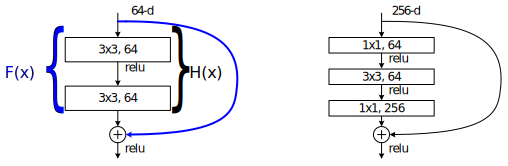
\includegraphics[width=0.85\linewidth]{resnet}
			\caption[ResNet blocks]{
				(\citet{resnet})
				\todo{Add \(\mathcal{H}(\ve{x})\) on the schema and small explanation.}
				\label{fig:resnet}
			}
		\end{figure}

		\todo{Show examples of extracted features for detection ? }

	%----------------------------------------------------------------------------------------

	\subsection{Region proposal network}\label{sec:frcnn_rpn}
		In order to bring the inference speed closer to real-time, \FRCNN{} improves on the bottleneck of previous approaches, namely the proposal of object candidates. Instead of relying on highly-engineered low-level features of super-pixels, the architecture reuses the convolutional feature map generated for the region classification step.

		This is achieved through another small, fully-convolutional network which is slided along the final layer of the feature map. The window at each location is projected into a lower dimensional feature that is used to predict \(k\) region bounds as well as \(k\) ``objectness'' scores. Each predicted region \(k_i\) is encoded as 4  coordinates \((x_1, y_1, x_2, y_2)_i\) that are \emph{relative} to a set of predefined boxes called \emph{anchors}. This mechanism allows the detection of multiple scales and aspect ratios in one pass through the network, thus avoiding the need of image pyramids and further reducing the computational cost.

		For training the RPN, the following loss function has to be minimised:
		\begin{equation}\label{eq:rpn_loss}
		L(\{p_i\}, \{t_i\}) = \frac{1}{N_{\cls}}\sum_i L_{\cls}(p_i, p^{*}_i) + \lambda\frac{1}{N_{\reg}}\sum_i  p^{*}_i L_{\reg}(t_i, t^{*}_i);
		\end{equation}
		\(p_i\) represents the probability that anchor \(i\) is an object; \(p^{*}_i\) is the label of this anchor (\(1\) when it significantly overlaps a ground-truth box) and \(t_i, t^{*}_i\) encode the anchor's and ground-truth's coordinates, respectively.

		The loss jointly minimised  the ``objectness'' classification term \(L_{\cls}\) for an anchor \(i\) in the minibatch and the bounding box regression term \(L_{\reg}\); the two are balanced by the hyperparameter \(\lambda\). The regression term is only taken into account for positive anchors (\(p^{*}_i = 1\)), which are those overlapping a ground-truth box with an Intersection-over-Union (IoU) ratio above threshold \(\tau = 0.7\).

	%----------------------------------------------------------------------------------------

	\subsection{Training}\label{sec:frcnn_train}
		In addition to the RPN, the \FRCNN{} architecture also needs to classify the generated proposals. For this, it uses the Fast R-CNN architecture and trains both of them at the same time, as shown in \autoref{fig:faster_rcnn}. The forward pass generates box proposals that the classifier considers to be fixed for its training. This easy implementation ignores the gradients with regards to the coordinates of the proposal boxes, so it is only an approximation of the joint training procedure. However, its results are close to those obtained by alternating the training of the two networks, while being significantly faster.

		Instead of training the whole architecture from scratch, we gain significant time by using transfer learning and starting with a model that performs well on the ImageNet challenge. We replace its final softmax layer so that it only predicts among our two classes of interest: \texttt{text} or \texttt{background}.

		We hypothesize that the object / not-object distinction is easier to make for text detection in white background documents than it is for an ImageNet object. Therefore, we set hyperparameter \(\lambda = 2\) in order to give preference to the localisation loss. Moreover, in order to account for text's wide aspect ratio and relatively constant height in our documents, we generate similarly wide anchors (ratios \(\{2, 4, 6, 8, 10\}\)) with a limited set of scales (heights of \(\{50, 75, 100\}\)px). This further helps the box regression part to converge.

		We use the stochastic gradient descent (SGD) optimiser with momentum, on batches of 1 input image. Note, however, that a minibatch is formed of bounding boxes, so many candidates can be generated from a single input image and a set of anchors. Several hyper-parameters control the composition of the batches:
		\begin{description}
			\item[number of proposals (\(\mathit{value} = 300\))] How many object proposals are generated in each batch.

			\item[positive to negative ratio (\(\mathit{value} = 0.5\))] For a robust classification and convergence of ``objectness'' score, it is important that examples of both positive and negative candidates are generated.

			\item[positive IoU threshold (\(\tau_{+} = 0.7\))] An anchor is considered positive when \(\mathit{overlap}(\mathit{anchor}, \mathit{truthBox}) > \tau_+\). While \(0.7\) can be considered low for text objects (see \autoref{fig:overlap}), setting this value too high in the early stages leads to a lower number of positive candidate and slows down convergence of \(L_{cls}\).

			\item[negative IoU threshold (\(\tau_{-} = 0.3\))] Similar to \(\tau_{+}\), but for marking candidates as negative examples.

			\item[NMS confidence threshold (\(\mathit{value} = 0.0\))] When a candidate has a low confidence score, we can supress it from contributing to the loss. We effectively disable this filter because we want to force the network to give high-confidence predictions, therefore it should learn from all examples.

			\item[NMS IoU threshold (\(\mathit{value} = 0.7\))] When several proposals overlap each other, we should keep only one of them in order to encourage proposal's diversity. This parameter controls when we can consider that a proposal is redundant to another one, in terms of their overlap.

		\end{description}

		On every experiment we monitor the training progress by intermittently evaluating the model on a validation dataset of images from the same category. The training is stopped once there is no significant improvement for more than two epochs, despite a decreasing learning rate.


%========================================================================================


\section{Training data}\label{sec:detection_data}
	Given the large number of parameters in deep neural networks (\(\approx 6 \times 10^8\) for \RESNET{}), it is clear that large amounts of training data are needed. Since this is lacking for our project, we must find alternative sources of handwritten text, ideally in the same language as the documents, i.e. French. Moreover, as was noted in \autoref{sec:challenges}, our documents have a specific format and less than optimal quality. The rest of the section shows how we transition from the clean and neat handwriting database to a format that helps the algorithm generalise to our use case.

	%----------------------------------------------------------------------------------------

	\subsection{The RIMES database}\label{sec:rimes}
		The RIMES database \citep{rimes} is the result of a huge data collection effort by the French ministries of defense and research, which was set up in order to create a new, consistent database of handwritten text. Its novelty was that it also included mixed pages, with handwritten and printed text, as well as being almost completely unconstrained with regards to the content of the text.	It contains more than \(50\,000\) handwritten words that are made available individually, or in lines (more than \(9000\)), or in paragraphs (more than \(1500\)).

	%----------------------------------------------------------------------------------------

	\subsection{Collage of paragraphs}
		For the first training session, we used images of paragraphs from the database along with their segmentations into lines as labels. To make them resemble the format of the documents, we juxtaposed two or three paragraphs picked at random from the database. These were corrected for rotation and augmented with borders, similarly to the sections in a document (\autoref{fig:collage}). We generated \(3500\) examples for training and \(500\) for validation.

		In our comparisons, we will refer to this dataset as \ds{Collage}.

		\todo{We noted that this model performs well on validation, but the transfer does not generalise. The cause is the sampling of negative anchors, which are almost inevitably white. In addition, the line lengths do not vary too much, neither the heights (which are bigger than our text) therefore bad regression of bboxes.}

		\begin{figure}
			\centering
			\begin{subfigure}[c]{\textwidth}
				\includegraphics[width=\textwidth]{collage_3}
				\caption{}
				\label{sfig:collage_clean}
			\end{subfigure}
			\vspace{1em}

			\begin{subfigure}[c]{\textwidth}
				\includegraphics[width=\textwidth]{collage_3_detected}
				\caption{}
				\label{sfig:collage_detect}
			\end{subfigure}
			\caption[\ds{Collage} dataset]{
				The \ds{Collage} dataset.
				\subref{sfig:collage_clean}: Example of generated collage document with 3 juxtaposed paragraphs.
				\subref{sfig:collage_detect}: The detection performed on such a document, with ground-truth in black and detection result in green.
			}
			\label{fig:collage}
		\end{figure}

	%----------------------------------------------------------------------------------------

	\subsection{Filled templates}
		%----------------------------------------------------------------------------------------
		% subsubsection: general description

			To address the limitations of the \ds{Collage} dataset, we propose to generate documents which resemble more the real ones. To this end, we fill accident statement templates of 4 different styles with handritten text from a database. This results in realistic looking documents while saving the high cost of manual labelling.

			A template is formed by adding input placeholders to an empty document (\autoref{fig:template}). These correspond to the standard places that the users need to fill as well as non-standard places where users regularly add information. To increase the variation of the data, only a subset of the placeholders are filled on each template instance and the input text is shifted to the right of the placeholder's edge with a random amount. We investigate two possible text sources for filling the placeholder.

			The first one consists of images of \emph{individual} words from the RIMES database. These are generally shorter than the placeholders, so we would need to concatenate several words to resemble the real data. Since the word order was lost when constructing the database, this has the disadvantage that the lines formed this way do not follow any sentence structure. Furthermore, handwriting styles from multiple authors would be combined on the same line and in the same document section.

			The second source of text consists of images of text lines from the same database. This addresses the problems of word concatenation, but introduces another difficulty: the lines usually do not fit inside the placeholders, so they need to be cut. However, thinking forward about the text transcription part, we immediately realise that in order to have reliable \((\mathtt{image}, \mathtt{label})\) pairs, we must ensure line images are split \emph{only between the words}. We use the following algorithm to detect good splitting points in image \(\ma{I}\):\footnote{\todo{use some ``algorithm'' package here; although these are quite fixed}} % https://tex.stackexchange.com/questions/172399/how-to-write-sentences-in-an-algorithm-in-latex https://tex.stackexchange.com/questions/142922/how-to-align-text-within-an-algorithm-environment
			\noindent\begin{minipage}{\linewidth}
			\begin{enumerate}
				\item use the line transcription labels to find the number of words \(n\)
				\item project the image columns horizontally, accumulating their sum into \[
					\ve{p}[c] = \sum_r \ma{I}[r,c]
				\]
				\item find the continuous runs of zero \(\ve{z} = \{ (i, j) \mid \ve{p}[k] = 0, \forall k \in [i, j] \}\); these correspond to gaps between letters (marked in red in \autoref{fig:baseline_ok})
				\item take \(n\) widest gaps \(\ve{z}'\) from \(\ve{z}\), with the gap width \(w := j - i\)
				\item split at columns \(c_k = \frac{j_k - i_k}{2}, \forall (i_k, j_k) \in \ve{z}'\).
			\end{enumerate}
			\end{minipage}
			\\

			To avoid placeholders filled with very short words, we add multiple words to the same placeholder until it is at least 75\% filled. Note that unlike the first text source, these words come in order from the original line, splitted by the above algorithm. Moreover, lines come sequentially from the same paragraph, so there is writer consistency for a good part of a template, just like in the real world.

			\begin{figure}
				\centering
				\includegraphics[width=\linewidth]{template_empty}
				\caption[Document template]{An empty document template. Note that the placeholders are slightly bigger than the location for text entry in order to allow text that goes out of bounds. Also, there are placeholders in places that do not correspond to any field, which matches how people use these documents.}
				\label{fig:template}
			\end{figure}

		%----------------------------------------------------------------------------------------

		\subsubsection{Baseline detection}
			When humans fill a statement template, the baseline of their handwriting lies roughly on an indicated line.  We purposely set the placeholder's bottom edge on this line in the interest of aligning the text image in a similar manner. Then we use the following simple algorithm to find the baseline row \(r_b\) of a text image \(\ma{I}\) of size \(H \times W\) (\autoref{fig:baseline}) :
			\noindent\begin{minipage}{\linewidth}
			\begin{enumerate}
				\item project the rows of the image by averaging the pixel values: \[
					\ve{p}[r] = \frac{1}{W} \sum_c I[r,c]
				\]
				\item let \(m = \operatorname{median}(\ve{p})\)
				\item the baseline is the first row \(r_b\) where \(\ve{p}[r_b] > m\), \(b = \overline{n, 1}\).
			\end{enumerate}
			\end{minipage}\\

			This algorithm works well as long as a few assumptions hold. First, the text image has to be horizontal. In case it is not (see \autoref{fig:baseline_skewed}), we deskew it by rotating with the average angle of Hough lines. Second, the input line has to be correctly segmented vertically. As a counter example, \autoref{fig:baseline_segmentation} shows that due to another text line present in the same image it is difficult to segment the words correctly. Fortunately, the database does not contain many examples that break these assumptions and we can reject tokens resulted from a failed segmentation based on their length.

			\begin{figure}[h!]
				\centering
				\begin{subfigure}{\linewidth}
					\includegraphics[width=\linewidth]{baseline_ok}
					\caption{Good and clean horizontal image}
					\label{fig:baseline_ok}
				\end{subfigure}

				\begin{subfigure}{\linewidth}
					\includegraphics[width=\linewidth]{baseline_skewed}
					\caption{Skewed image}
					\label{fig:baseline_skewed}
				\end{subfigure}

				\begin{subfigure}{\linewidth}
					\includegraphics[width=\linewidth]{baseline_segmentation}
					\caption{Badly segmented image, with slanted text}
					\label{fig:baseline_segmentation}
				\end{subfigure}
				\caption[Baseline and tokens]{Detection of the baseline and the tokens in a text image.}
				\label{fig:baseline}
			\end{figure}

		%----------------------------------------------------------------------------------------

		\subsubsection{Filling with generator}
		\startToDo
			Should we actually mention this, given that we only introduce the generator later, for transcription ?

			Also, no tests for \FRCNN{} + Generator data, only \CTPN{}. So, should I include it here or later in CTPN section ?
		\stopToDo

		%----------------------------------------------------------------------------------------

	%----------------------------------------------------------------------------------------

	\subsection{Results}\label{sec:frcnn_results}
		\begin{figure}[h!]
			\centering
			\begin{subfigure}{.49\linewidth}
				\includegraphics[width=\linewidth]{frcnns_by_iou.png}
				\caption{}
				\label{fig:frcnns_by_iou}
			\end{subfigure}
			\begin{subfigure}{.49\linewidth}
				\includegraphics[width=\linewidth]{frcnns_by_scores.png}
				\caption{}
				\label{fig:frcnns_by_scores}
			\end{subfigure}
			\caption[\FRCNN{} results]{\todo{...}}
			\label{fig:frcnn_results}
		\end{figure}



%========================================================================================


\section{Connectionist Text Proposal Network}\label{sec:ctpn}
	% http://i.cs.hku.hk/~kykwong/publications/wliu_bmvc16.pdf This has a good simple explanation of ResNet and LSTM and what-not


	\todo{Compare and contrast with \FRCNN{} RPN. Also, we use the VGG, because it came with the network}
%----------------------------------------------------------------------------------------


%========================================================================================


\section{Results}\label{sec:detection_results}
	This gives an overview of object detection evaluation:

	% https://www.researchgate.net/profile/Rangachar_Kasturi/publication/220928471_Performance_Evaluation_of_Object_Detection_Algorithms/links/54c91dd00cf25087c4ec62fd.pdf

	this evaluates text detection in 2 simple numbers (P, R), in terms of pixels

	http://vision.soic.indiana.edu/papers/textevaluation2000das.pdf

	\todo{Evaluation method: goal-directed approach = couple with text recognizer; see % http://citeseerx.ist.psu.edu/viewdoc/download?doi=10.1.1.332.3461&rep=rep1&type=pdf
	}
	\todo{
		Compare all \FRCNN{} with \CTPN{}
	}


%----------------------------------------------------------------------------------------

% %!TEX root = ../main.tex

\chapter{Transcription}\label{ch:transcription}

This chapter is dedicated to the problem of offine handwriting recognition, that is, given an image of a text line, find the corresponding characters and words. Although some may consider it a solved task, since many approaches achieve very good performance on a wide variety of corpora (see \autoref{sec:related_transcription}), we remind the reader that our use case poses several challenges that are not present in the controlled environments of academic contests (\autoref{sec:challenges}). Of these, we summarise the most important ones:
\begin{description}
	\item[unbefitting writing conditions] The documents are completed in a rush, soon after an accident, with no proper support structure for writting and with few format restrictions.

	\item[unconstrained recognition] Statements include text which does not admit a vocabulary for correction, such as phone numbers and license plates.

	\item[lack of annotated data] As in the case of detection, we started the project having only a database of images and no useful annotations.
\end{description}

The chapter first introduces the \CRNN{} architecture \citep{CRNN}, which has become almost a standard for optical character recognition in the recent years. Then, \autoref{sec:transcription_experiments} presents several experiments for training, including various methods of data generation. Each new experiment tries to address the weaknesses of the previous one, in a quest of reproducing the great results obtained on clean databases. Finally, we explore the potential of an attention-based architecture coupled with the same training data in \autoref{sec:attention} and present an overview of the obtained results in \autoref{sec:transcription_results}.



%========================================================================================

\section{Convolutional Recurrent Neural Networks}\label{sec:crnn}

	%--INTRO --------------------------------------------------------------------------------

		Text transcription has preoccupied researchers for a very long time. Therefore, a large amount of ideas have been tried in order to solve this problem, of which we mention a few in \autoref{sec:related_transcription}. One of the challenges of text resides its wide variation of appearance. For example, a free font website such as \url{http://www.1001fonts.com/} currently lists approximately 9500 different typefaces. Moreover, it is believed that each person has a completely unique handwriting, which is why this is still commonly used a signature. This highlights the importance of being able to represent images of text robustly, or, in other words, to extract good features that distinguish well among characters. As was previously stated, convolutional neural networks have proved very effective in this task time and again, so it is natural to use them as a first stage in a transcription architecture.

		Another peculiarity of text, which we have also mentioned in the detection chapter, is given by its sequential aspect. Few neural network architectures support arbitrarily-sized input. Of these, the recurrent neural network (RNN) has become a standard since it models well sequences of any type.

		The Convolutional Recurrent Neural Network (\CRNN{}) architecture uses the two approaches above in a unified framework to transcribe text from natural images. Considering that it achieved state-of-the-art performance in such a challenging task, we believe it is suitable for our use case as well, which is why we focused most of our efforts in this direction. Next, we detail its inner workings as they are crucial in devising our experiments.


		\begin{figure}\begin{tabular}{|c|c|}
			% \footnotesize
			\hline
			\textbf{Type} & \textbf{Configurations}						\tabularnewline	\hline
																																				\hline
			Transcription & - 																\tabularnewline	\hline
			Bidirectional-LSTM & \#hidden units:256						\tabularnewline	\hline
			Bidirectional-LSTM & \#hidden units:256						\tabularnewline	\hline
			Map-to-Sequence & - 															\tabularnewline	\hline
			BatchNormalization & - 														\tabularnewline	\hline
			Convolution & \#maps:512, k:$2\times2$, s:1, p:0	\tabularnewline	\hline
			MaxPooling & Window:$1\times2$, s:2								\tabularnewline	\hline
			Convolution & \#maps:512, k:$3\times3$, s:1, p:1	\tabularnewline	\hline
			BatchNormalization & - 														\tabularnewline	\hline
			Convolution & \#maps:512, k:$3\times3$, s:1, p:1	\tabularnewline	\hline
			MaxPooling & Window:$1\times2$, s:2 							\tabularnewline	\hline
			Convolution & \#maps:256, k:$3\times3$, s:1, p:1	\tabularnewline	\hline
			BatchNormalization & - 														\tabularnewline	\hline
			Convolution & \#maps:256, k:$3\times3$, s:1, p:1	\tabularnewline	\hline
			MaxPooling & Window:$2\times2$, s:2								\tabularnewline	\hline
			Convolution & \#maps:128, k:$3\times3$, s:1, p:1	\tabularnewline	\hline
			MaxPooling & Window:$2\times2$, s:2 							\tabularnewline	\hline
			Convolution & \#maps:64, k:$3\times3$, s:1, p:1		\tabularnewline	\hline
			Input & $W\times32$ gray-scale image 							\tabularnewline	\hline
		\end{tabular}\par
		\caption[\CRNN{} architecture]{\todo{Note different from paper}}\label{fig:crnn_architecture}
		\end{figure}

	%----------------------------------------------------------------------------------------
	\subsection{Feature extraction}
		The first part of the \CRNN{} architecture consists of a custom 7-layer CNN that transforms the input image into a sequence of high-level features. This is similar to well-known architectures, as it alternates convolutional and pooling layers (\autoref{fig:crnn_architecture}). A few particularities are important to be noted.

		First, the input is pooled differently on the vertical dimension than on the horizontal one. For the former, 4 windows of height 2 are used. As a result, an input of height 32 becomes a feature map of height 2. In order to feed this to the RNN, the features on the same column are concatenated into a single vector. Then, the nework performs horizontal pooling only twice with a window of width 2. This ensures the receptive field does not become too wide and can still distinguish very narrow characters such as \{\texttt{l,i,1}\}. The network is fully convolutional, which allows inputs of any size to be processed. However, since the columns become features of the RNN, the height should be standardised. This design is well suited for images of text which are bounded vertically, but not horizontally.

		Second, the network uses batch normalisation \citep{batch_norm}, which is standard practice in recent times since it improves the performance and the stability of the network. This works by replacing the activations \(\ve{H}\) of a layer with their normalised counterparts \(\ve{H}'\), which become input for the next layer: \[
			\ve{H}' = \gamma \frac{\ve{H} - \ve{\mu}}{\ve{\sigma}} + \beta,
		\]\footnote{\todo{make miu and sigma vectors}} where \(\mu\) is a vector of means of all neurons and \(\sigma\) a vector of their standard deviations. The learnable parameters \(\gamma\) and \(\beta\) ensure the network does not lose expressive power by allowing convergence towards any mean and standard deviation. Overall, this also means that the composition of the batches is important, as we will see shortly.

		Finally, we use ReLU activations at each layer and bias terms for the convolution.

		%........................................................................................
		\subsubsection*{Input preprocessing}

			Input images are resized to have a heigth of 32px, while keeping their aspect ratio. As a result, their widths are different which makes it difficult to construct batch tensors. Therefore, we also define a standard input width of 250px and make sure all training images are narrower than this in the interest of avoiding horizontal deformation. Images that are shorter than the necessary width are duplicated horizontally up to this length. As opposed to zero padding the shorter images, this mechanism keeps a similar distribution of pixels across all batches. Note this does not produce bad training examples as we keep track of the original length when aligning the predictions and the labels.

\startToDo{}

	%----------------------------------------------------------------------------------------

	\subsection{RNN decoder}

	%----------------------------------------------------------------------------------------

	\subsection{Training}
		dropout

		alphabet encoding


	%----------------------------------------------------------------------------------------

	\subsection{Evaluation}
		edit distance

		lowercase, uppercase

		mention the TEST corpus and the thing with underscores

%========================================================================================

\section{Experiments}\label{sec:transcription_experiments}

	%----------------------------------------------------------------------------------------

	\subsection{Academic databases}
		RIMES lines, words, words with spaces + IAM

		show examples, and numbers

		Mention problems: writing style, different corpus (MAJ vs min vs ligatures + numbers, plates), lines

	%----------------------------------------------------------------------------------------

	\subsection{Generator}

		mention the success in OCR

		mention specific changes that we brought (no projection, no curved, random jitter, lines)

		subsubsection: scrapping fonts + elastic distortions

		results:  closer, but not enough doesn't know if it's a date or a number so D, 0, O

	%----------------------------------------------------------------------------------------

	\subsection{Corpus type}
		strategy 1: precondition the hidden state, like Karpathy
		Not working because not enough information. They were embedding a very rich feature into the space of the hidden state, whereas we merely ``tickle'' the hiddent state

		Strategy 2: add extra feature at all time steps

%========================================================================================

\section{Attention-based architecture}\label{sec:attention}
	biiig TODO

%========================================================================================

\section{Results}\label{sec:transcription_results}

		Show a table of each approach and the corresponding CER, and call it a day :)

\stopToDo{}



\bibliography{refs}             % this causes the references to be listed
\bibliographystyle{plainnat}       % see natbib for other possible values

% \include{chapters/appendix}

\end{document}
